
\frame{\partpage }
\begin{frame}[fragile]{Why mixing C++ and Python? - Two use cases}
    \note{
        \begin{itemize}
            \item \texttt{Ipython}-session loading a C++ wrapper
            \item Paraview uses Python as its internal scripting language
        \end{itemize}
        Only C++ from python will be covered in this talk.
    }
    \begin{center}
        \textbf{Calling C++ from python}
    \end{center}
    \begin{columns}[c]
        \begin{column}{0.49\linewidth}
            \begin{itemize}
                \item write performance critical code in C++
                \item reuse existing C++ libraries 
            \end{itemize}
        \end{column}
        \hfill
        \begin{column}{0.4\linewidth}
            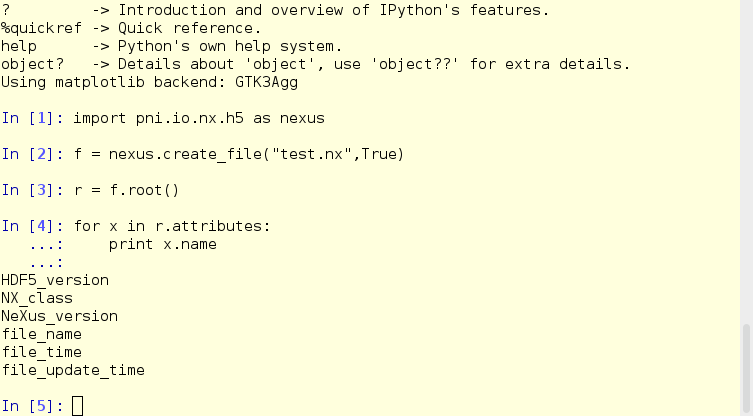
\includegraphics[width=\linewidth]{pics/ipython_screenshot.png}
        \end{column}
    \end{columns}
    
    \vspace{0.05\textheight}
    \begin{center}
        \textbf{Calling Python from C++}
    \end{center}
    \begin{columns}[c]
        \begin{column}{0.49\linewidth}
            Use Python as an embedded scripting language for a 
            C++ application
        \end{column}
        \hfill
        \begin{column}{0.4\linewidth}
            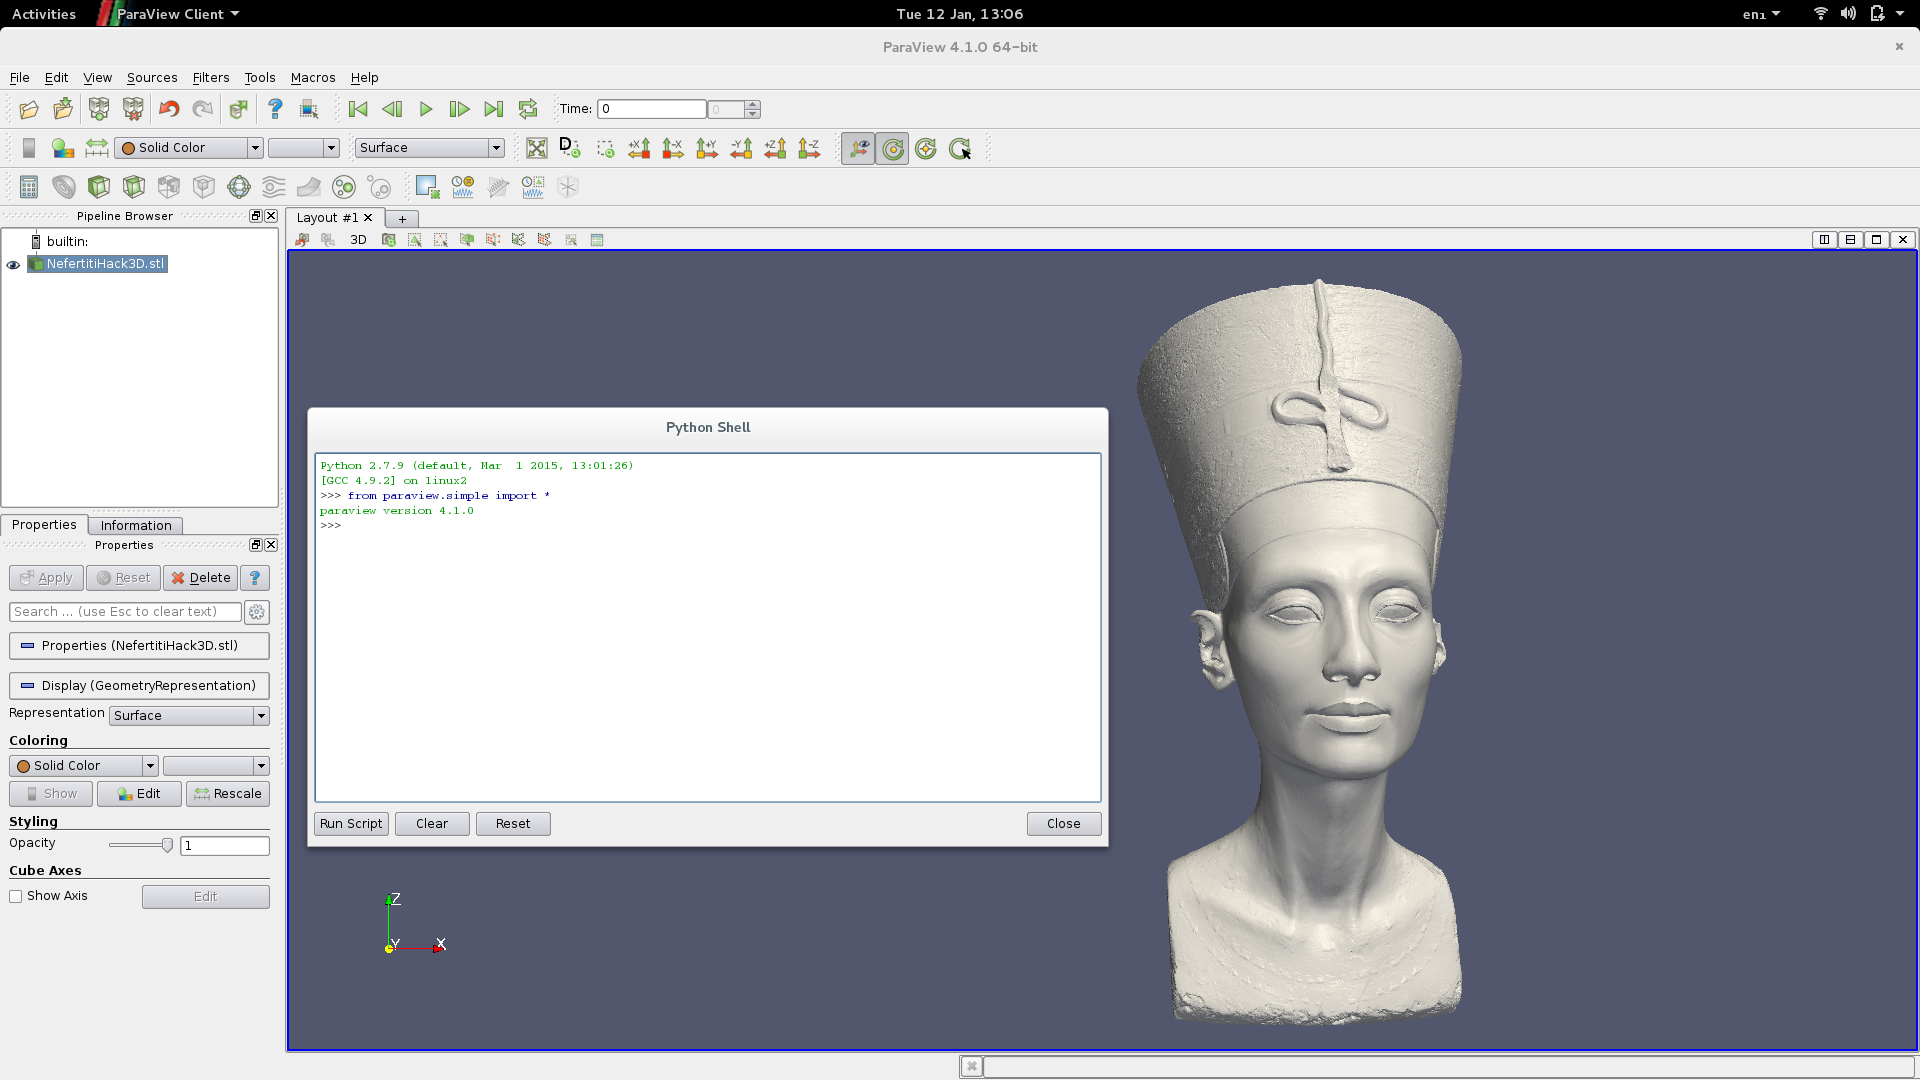
\includegraphics[width=\linewidth]{pics/paraview.png}
        \end{column}
    \end{columns}
    

\end{frame}

%%%===========================================================================
\begin{frame}[fragile]{Available technologies}
    \note{
        Our focus is on \texttt{boost::python}!
    }
    
    \begin{itemize}
        \setlength{\itemsep}{0.075\textheight}
        \item native Python C-API (do not use this until you have to)
        \item \texttt{boost::python} (part of the BOOST distribution)
        \item \texttt{cython} -- good for numerical applications
        \item \texttt{sheboken} -- used for instance with \texttt{pyside}
    \end{itemize}
\end{frame}

